\documentclass[a4paper, 12pt]{article}
\usepackage[total={17cm,25cm}, top=2.5cm, left=2.5cm, right=2.5cm,  includefoot]{geometry}
\usepackage[utf8]{inputenc}
\usepackage{array}
\usepackage{multirow}
\usepackage{hhline}
\usepackage{gensymb}
\usepackage{graphicx}
\graphicspath{ {} }
\usepackage[czech]{babel}
\usepackage{enumitem}
\usepackage{pdfpages}
\usepackage{amsmath}
\usepackage{verbatim}
\usepackage{listings}
\usepackage{hyperref}
\usepackage{amssymb}


\pagestyle{empty} % vypne číslování stránek




\usepackage[OT2,OT1]{fontenc}
\newcommand\cyr
{
\renewcommand\rmdefault{wncyr}
\renewcommand\sfdefault{wncyss}
\renewcommand\encodingdefault{OT2}
\normalfont
\selectfont
}
\DeclareTextFontCommand{\textcyr}{\cyr}
\def\cprime{\char"7E }
\def\cdprime{\char"7F }
\def\eoborotnoye{\char’013}
\def\Eoborotnoye{\char’003}


\begin{document}



\begin{titlepage}
\begin{center}
\noindent
\Large \textbf{České vysoké učení technické v Praze }\\ Fakulta stavební
\vspace{5cm}

\huge

%vložení loga cvut
\begin{figure}[h!]
	\centering
	
\includegraphics[width=7cm]{logo.png}
\end{figure}

\vspace{0.5cm}

Úvod do zpracování prostorových dat \\

\vspace{3cm}

\Huge  
Přírodní prvky okresu Strakonice\\

\vspace{2cm}

\Large
Bc. Michal Janovský \\
Bc. Petra Pasovská \\

\end{center}

\end{titlepage}




\pagestyle{plain}     % zapne obyčejné číslování
\setcounter{page}{1}  % nastaví čítač stránek znovu od jedné

\tableofcontents
\newpage


\section{Úvod}
Tato dokumentace je součástí semestrálního projektu v předmětu Úvod do zpracování prostorových dat pod vedením Ing. Martina Landy, Ph. D. Hlavním cílem projektu bylo vytvoření databáze, nad níž budou následně volány prostorové dotazy.\\
\\
Autoři si sami zvolili takové téma, které je zajímá a sami si vyhledávali zdroje. Jedním z hlavních cílů tohoto projektu je mimojiné prozkoumání jednotlivých zdrojů. Za tímto účelem bylo pro analýzu vybráno menší zájmové území - okres Strakonice (nebo Jihočeskký kraj??). \\
\\
Přírodní prvky byly zvoleny z toho důvodu, neboť autoři mají velmi kladný vztah k přírodě. Navíc v rámci přírodních prvků je prováděno velké množství analýz, díky čemuž je pro toto téma mnoho dat a je zde větší množství zdrojů, které mohou autoři prozkoumat.\\
\\
Výsledkem práce je databáze obsahující několik bodových, liniových a polygonových vrstev.

\clearpage
\section{Zdrojová data}
Pro tento projekt bylo použito několik zdrojů. 

\subsection{DIBAVOD}
Digitální báze vodohospodářských dat, zkráceně DIBAVOD, je referenční geografická databáze, která je součástí nadstavby ZABAGED (Základní báze geografických dat ČR - digitální topografický model území ČR odvozený z mapového obrazu Základní mapy České republiky 1:10 000). Primárně byla vytvořena pro tvorbu tématických kartografických výstupů s vodohospodářskou tematikou a tematikou ochrany vod. \\
\\
Obecně lze DIBAVOD považovat jako databázi podkladových dat pro kategorii vodstvo pro ZABAGED. Uživatel má možnost si zdarma stáhnout data ve formátu shapefile v několika podkategoriích, např. chráněná území, objekty na toku, záplavová území či měřící a kontrolní mmísta povrchových vod. 

\begin{figure}[h!]
	\centering
	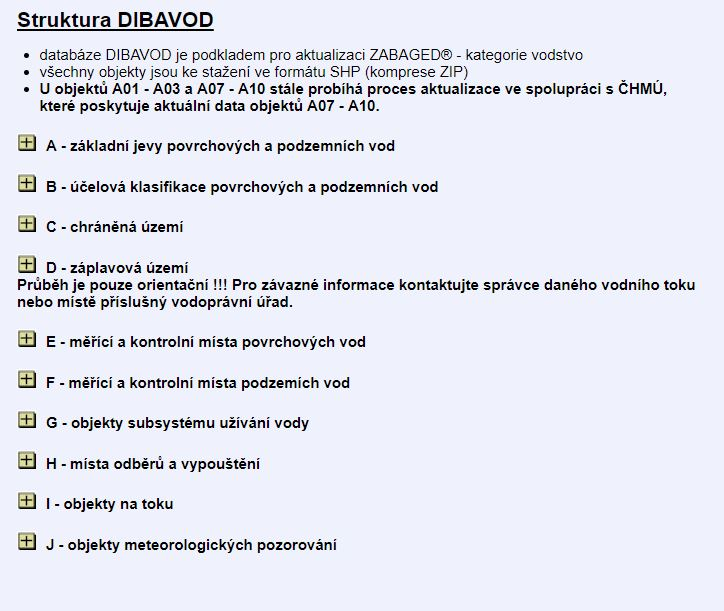
\includegraphics[width=13cm]{pictures/dibavod.jpg}
\end{figure}

\subsection{OpenStreetMap}
OpenStreetMap je projekt, jehož cílem je tvorba volně dostupných geografických dat a následně jejich vizualizace do podoby silniční mapy, uliční mapy měst atd. Tato vektorová data jsou poskytována pod licencí Open Database Licence. \\
\\
Jedná se o taková zdrojová data, která může kdokoliv upravit. Díky tomu se na tvorbě může podílet v podstatě kdokoliv, v současné době navíc existují i pluginy, které umožňnují stáhnutí OMS do Garminu či smartphonů. 

\begin{figure}[h!]
	\centering
	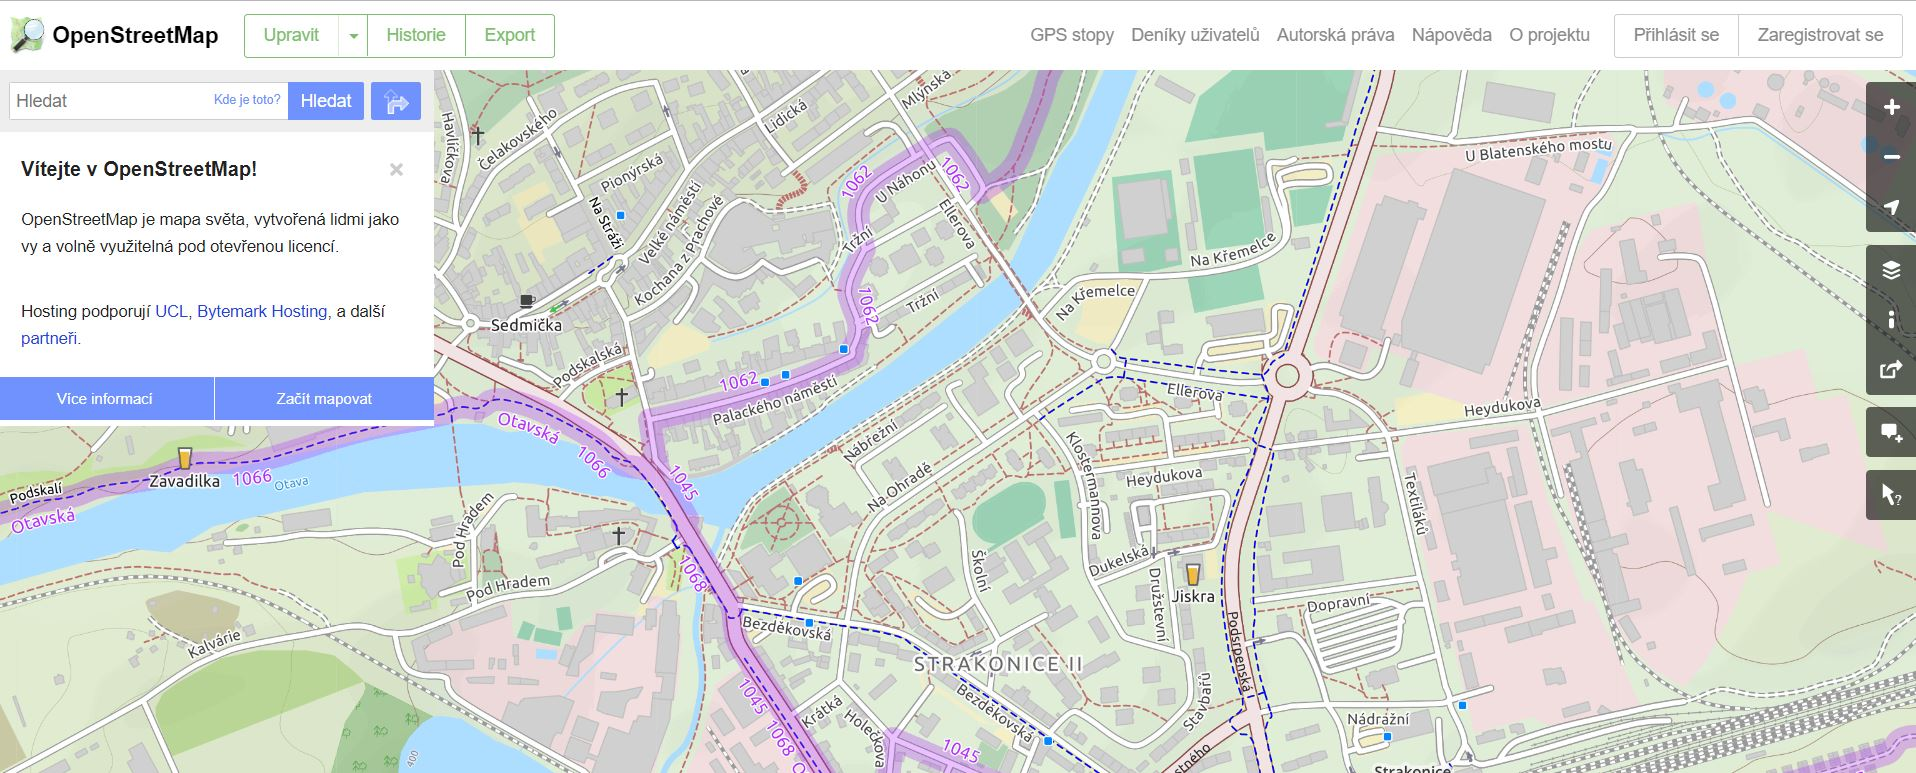
\includegraphics[width=14cm]{pictures/osm.jpg}
\end{figure}


\subsection{ArcČR 500}
ArcČR 500 je digitální vektorová geografická databáze České republiky. Data vznikla ve spolupráci ARCDATA Praha, s.r.o., Zeměměřického úřadu a Českého statistického úřadu. Data jsou pro uživatele k dispozici zdarma. \\
\\
Data lze rozdělit do tří hlavních složek - Administrativní členění, Geografické prvky a Klady a sítě. Pro projekt byly zahrnuty jen určité vrstvy z kategorie Geografické prvky. 

\begin{figure}[h!]
	\centering
	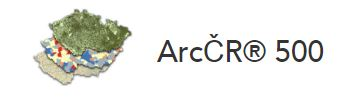
\includegraphics[width=8cm]{pictures/arccr.jpg}
\end{figure}

\subsection{AOPK ČR}
Agentura Ochrany Přírody a Krajiny ČR nabízí datové sady týkající se národně i mezinárodně chráněných územích či druzích, památných stromech, biotopech, rezervacích, geoparcích či mokřadech. Data jsou v souřadnicovém systému WGS84 a organizace nabízí řadu formátů, ve kterých lze data stáhnout.\\
\\
Agentura spadá pod Ministerstvo životního prostředí a v roce 2017 získala ocenění na evropské konferenci INSPIRE ve Štrasburku. 

\begin{figure}[h!]
	\centering
	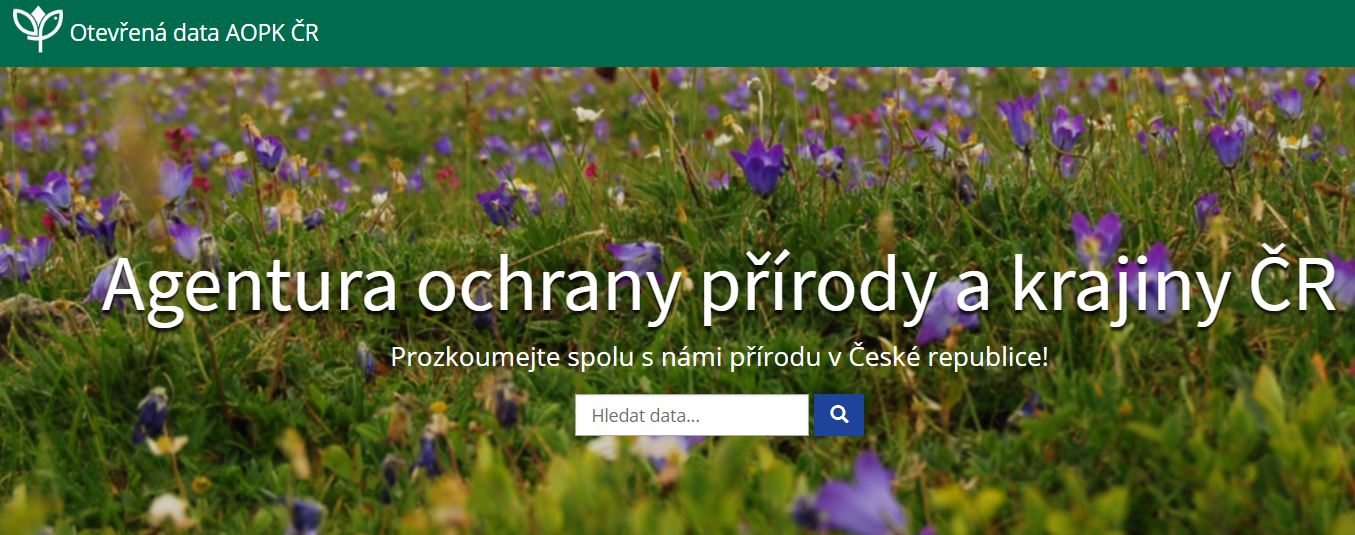
\includegraphics[width=12cm]{pictures/aopk.jpg}
\end{figure}

\section{Software}
QGIS? atd


\section{Analýza dat??}
zpracování, vrstvy atd

\section{Prostorové dotazy}

\section{Závěr}

\clearpage
\section{Reference}

\begin{enumerate}
\item  Presentation about convex and concave polygons [online][cit. 21.10.2018]. \\
Dostupné z: https://slideplayer.com/slide/6161031/  \\


\end{enumerate}
\end{document}



 